\documentclass{article}
\usepackage[utf8]{inputenc}

\usepackage{enumitem}
\usepackage{graphicx}
\usepackage{subcaption}
\usepackage{float}
\usepackage{amsmath}
\usepackage{amssymb}
\usepackage{setspace}
\usepackage{xfrac}
\usepackage{indentfirst}
\usepackage{tikz}
\usepackage{hyperref}
\usetikzlibrary{positioning, fit, calc, arrows,shapes.gates.logic.US,shapes.gates.logic.IEC,}
\usepackage[siunitx, RPvoltages]{circuitikz}

\usepackage{enumitem}

\title{ECE350 Final Review - Cramming Carnival Worksheet}
\author{Author: Members of HKN}
\date{}
\newcommand{\dd}[1]{\mathrm{d}#1}

\usepackage[makeroom]{cancel}
\usepackage[letterpaper, portrait, margin=1in]{geometry}
\usepackage{graphicx}

\pagenumbering{arabic}

\begin{document}

\maketitle

\section{Fiber Optics}
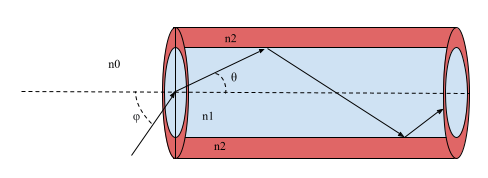
\includegraphics{figures/Optical Fiber Diagram.png}
The diagram above shows an Optical Fiber that is hit with a beam of light that enters the core(blue) of the fiber optic cable. The refractive index for the core $n_{1}=1.66$, the refractive index for the cladding(red) $n_{2}=1.63$, and the refractive index for air $n_{0}=1$. The wavelength of the light shown is $1200 nm$.

\begin{enumerate}[label=(\alph*)]
    \item {Find the maximum value of $\varphi$ such that the wave is contained within the core(i.e., there is Total Internal Reflection when the wave in the core hits the cladding).}
    
    \item {For the following questions, the Optical Fiber is now given a coating around the cladding with a refractive index $n_{3}=1.7$, $\varphi=10^{\circ}$, and we are operating in TE mode.}
    \begin{enumerate}[label=(\roman*)]
        \item {Find the angle of incidence of the wave in the core onto the cladding.}
        \item { What should the width d of the cladding be such that the transmittance is .0001 at the coating that surrounds the cladding?}
        \item {What is the angle of incidence of the wave transmitted through the coating?}
    \end{enumerate}
\end{enumerate}

\section{Waveguide Warm Up}
A parallel plate waveguide is filled with a dielectric with $\varepsilon=16*\varepsilon_{o}$. What is the spacing $a$, such that $5.5$ GHz is equal to $90\%$ of the $TE_{3}$ mode cutoff frequency?


\section{Finding modes}
A given parallel plate waveguide contains an air-filled region with a plate separation $a = 10$ cm. Find the propagating $TE_{m}$ modes for a frequency of 5.5 GHz, and for each mode determine $f_{c}$, $\lambda_{g}$, and $\theta$.

\section{Guided Waveguides}
We have a parallel plate waveguide that is filled with a dielectric with $\varepsilon=4*\varepsilon_{o}$. A signal frequency of 280 Mhz is propagating in the Waveguide. We have found that for the $TE_{2}$ mode the phase velocity is $v_{p} = 1.5*c$. Using this information we want to find the guided wavelength of $TM_{1}$ mode.

\begin{enumerate}[label=(\alph*)]
    \item {Find the width, $a$, of the waveguide.}

    \item {Find the phase velocity, $v_{p}$, of the $TM_{1}$ mode.}

    \item {Find the guided wavelength, $\lambda_{g}$, of the $TM_{1}$ mode.}

\end{enumerate}

\section{Disruptive Doppler}

Shomik is carrying a $\hat{z}$-polarized short dipole antenna, which is driven by an input current $i(t) = I_o cos(\omega t)$, where $\omega = 6 \cdot 10^9$ rad/s. Shomik is moving with the trajectory $(x, y, z) = (400 + 50t, 200 + 10t, t^2)$. Grant, moving with a trajectory of $(x, y, z) = (200 + 70t, 200 + 90t, t^2)$, is carrying another $\hat{z}$-polarized short dipole antenna which is displaying an open circuit voltage with a time-varying carrier phase $\Phi(t)$ in response to the field incident from Shomik's dipole. Assume free-space propagation for this problem.

\begin{enumerate}[label=(\alph*)]
    \item Express the carrier phase $\Phi(t)$ explicitly in terms of $\omega$ and $t$. Hint: Shomik's dipole radiates a spherical wave of the form $cos(\omega t - kr)$. Hint 2: Be smart about your coordinate system choice.

    \item Given that $\omega' = \frac{\partial \Phi}{\partial t}$, what is the Doppler frequency shift $\omega' - \omega$ of Grant's open-circuit voltage at $t = 0$?

    \item What is the Doppler frequency shift $\omega' - \omega$ of Grant's open-circuit voltage at $t = 10$?

    \item Find the time-point(s) at which the Doppler frequency shift $\omega' - \omega$ is zero. What is the physical significance of these time-points? How many such time-points are there?

    \item Qualitatively, what is the behavior of the Doppler frequency shift at the limits $t \longrightarrow \infty$ and $t \longrightarrow -\infty$ (i.e. constant? linear? quadratic?)? Name the approximation that can you use in these cases (you've seen it before in ECE350!).

    \item Are the calculations above relativistically correct?

\end{enumerate}

\newpage

\section{Clingy Conductors}

\begin{center}
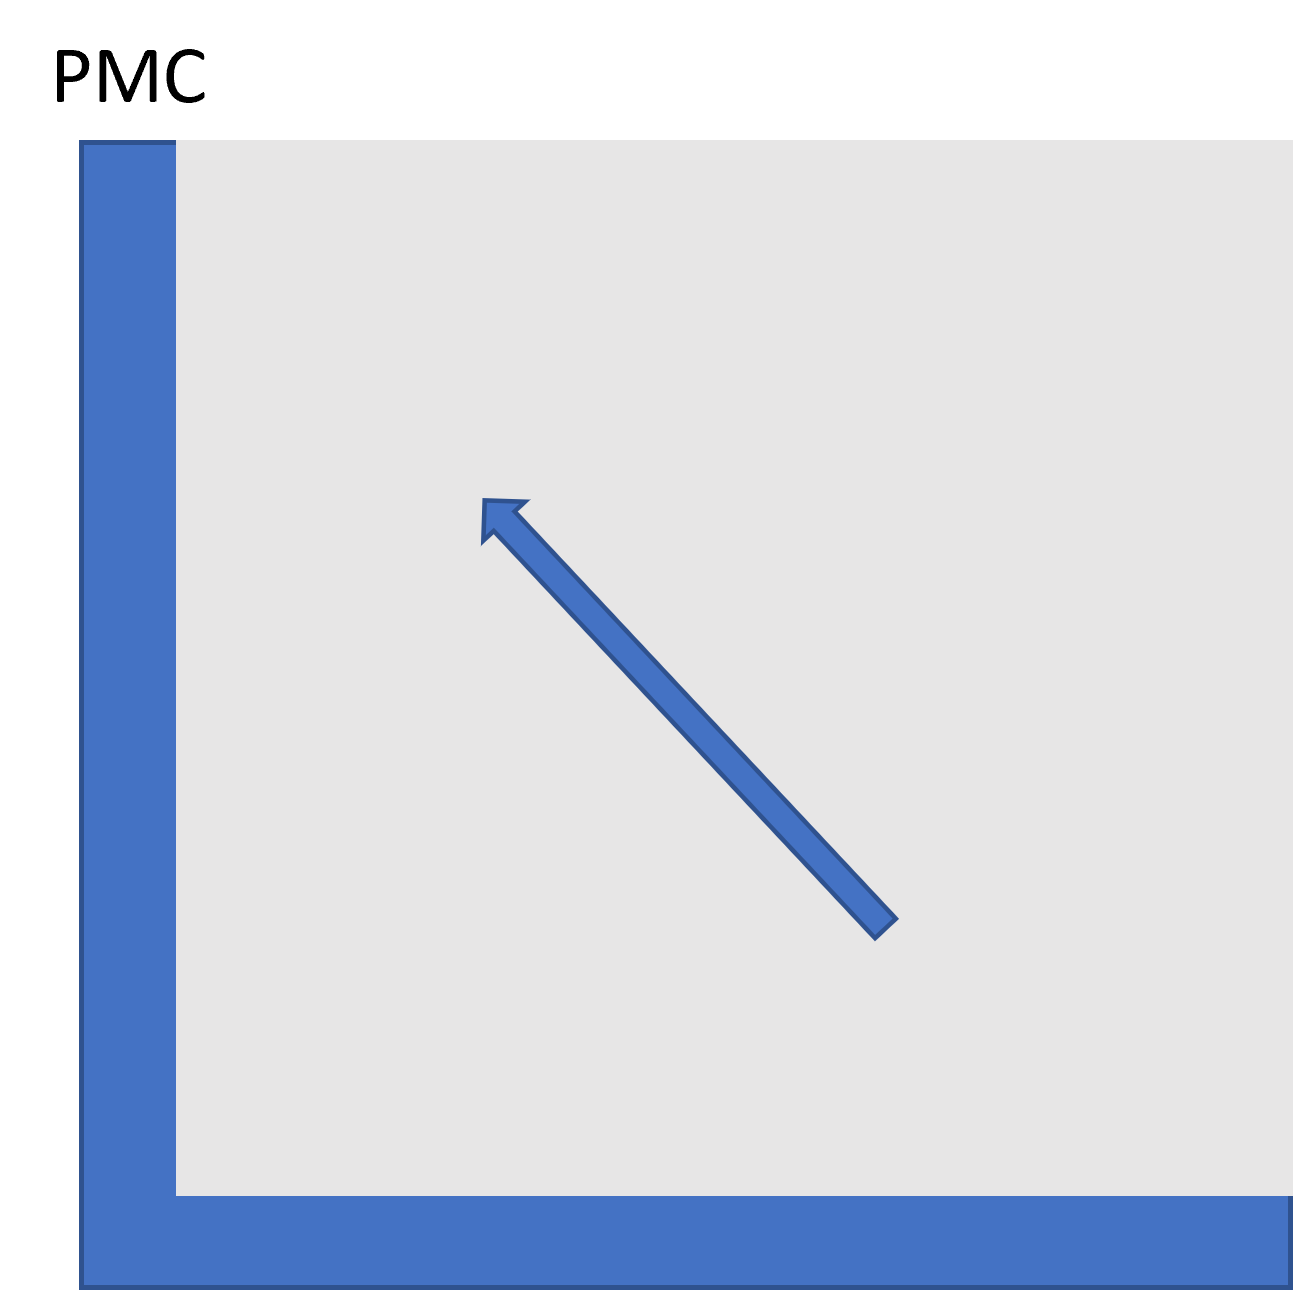
\includegraphics[width=0.5\textwidth]{figures/PMC Prompt.jpg}
\end{center}

Given the situation above, sketch the three image antennas resulting from the perfect \textbf{magnetic} conductor (PMC) (shown as the blue rectangles on the boundary) based on image theory. Recall that a PMC enforces the boundary condition that the tangential B field is zero (what does a PEC do instead?)

\section{Devious Duality}

\begin{enumerate}[label=(\alph*)]
    \item A line of negative charges sit on the $x = 0$ axis. The charges have a density of $\lambda$ charges per meter. What is the electric field as a function of position given off by these charges? What is the magnetic field as a function of position given off by these charges?
    
    \item You decide to now start travelling at $v = 0.5c$ in the $+\hat{x}$ direction. The charges now look like they are travelling at $0.5c$ in the $-\hat{x}$ direction. From your point of view, what is the electric field as a function of position given off by these charges? From your point of view, what is the magnetic field as a function of position given off by these charges?
    
    \item Points of view do not affect what is really happening. So what is the underlying truth?

\end{enumerate}

\newpage

\section{Rigid Reciprocity}

Let $\rho_1$ be a static charge distribution over free space with a corresponding potential distribution $\phi_1$, and $\rho_2$ be a static charge distribution over free space with a corresponding potential distribution $\rho_2$. 

\vspace{3mm}

Given Green's second identity on scalar functions:

\[
\int_U (\psi\nabla^2\varphi - \varphi\nabla^2\psi) dV = \oint_{\partial U}(\psi\nabla\varphi - \varphi\nabla\psi)\cdot dS
\]

prove Green's reciprocity theorem:

\[
\int \rho_1\phi_2 dV = \int \phi_2\rho_2 dV
\]

Note: The integral above is taken over $\textbf{all of free space}$. $\partial U$ represents the boundary of the set $U$.


\section{Peanut Butter Dispute}

Shomik and Grant are very angry with each other (something about peanut butter apparently). Shomik gets on his spaceship and travels away from Earth at a velocity of $0.6c$.  At the same time, Grant gets on his spaceship and travels away from Earth in the opposite direction at a velocity of $0.6c$. In the meantime, Shomik and Grant continue to send curse words and insults to each other using a radio with a frequency of $\omega$. The signals they send take the form of $Acos(\omega t)$, where $A$ is some (varying) amplitude.

\begin{enumerate}[label=(\alph*)]
    \item What is the frequency of the communication when detected from Earth?
    
    \item What is the frequency of Grant's communication as detected by Shomik?
    
    \item Using the normal formulae for velocity addition, how fast is Grant moving away from Shomik? Is this correct?
    
    \item Grant realizes that Shomik is not receiving his messages properly. What frequency must Grant use so that Shomik detects the frequency $\omega$?

\end{enumerate}

\newpage

\section{Time-Bender}

Shomik continues to send messages to Grant of the form $Acos(\omega t)$, which means that Grant receives them with the form $Acos(\omega' t - k'x) = Acos(\omega' t - k'vt) = Acos(\omega' \left(1 - \frac{v}{c} \right) t)$. Note that $\frac{\omega}{k} = c$ always in a vacuum, so if $\omega$ changes, then $k$ must also change. Also note the direction of our $x$-axis.

Grant now resorts to mocking Shomik instead. Grant then sends the exact same message back at the exact frequency that he received it at, aka $\omega'$. Shomik then receives his own message at frequency $\omega''$, enraging him further.

For this problem, assume that Grant is moving away from Shomik at velocity $v$. Be \textbf{extremely} careful about what point of view you are using. Really put yourself into Shomik's or Grant's shoes.

\begin{enumerate}[label=(\alph*)]
    \item At what velocity is Shomik moving away from Grant? (Yes, this is trivial.)
    
    \item What is $\omega'$, and $\omega''$? Express them as functions of $\omega$. Hint: Do problem 1 first.

    \item From Grant's point of view, what is the form of signal sent out by Grant? Write it out in the same format as provided (a cosinusoidal), although set $x = 0$ since Grant is always at the origin (from Grant's point of view). Leave you answer in terms of $\omega'$.

    \item From Shomik's point of view, what is the form of signal sent out by Grant? Write it out in the same format as provided (i.e. simplify your answer so that it does not use any version of $k$). Leave your answer in terms of $\omega''$.

    \item However, the signals in part (d) and part (e) must be the same signal - Grant and Shomik are just calling it different things. This is a fundamental postulate of physics: One's point of view \textbf{\textit{CANNOT}} affect the underlying truth (for if it did, this must be a single correct point of view, which feels very bad). Therefore, the solutions of (d) and (e) must be set equal to each other.
\end{enumerate}

\section{Space-Bender}

The above result has profound consequences. For this problem, assume that Grant is moving away from Shomik, from Shomik's point of view, at $v$.

\begin{enumerate}[label=(\alph*)]
    \item How fast is Shomik moving away from Grant in Grant's point of view? (Yes, this is trivial.)
    
    \item Given this conclusion and the conclusion of the previous part, what other quantity must be changing as we switch from Shomik's point of view to Grant's point of view? Express the quantity from Grant's point of view in terms of the quantity from Shomik's point of view.
\end{enumerate}

\newpage

\section{Dispersion Relation}

Shomik and Grant finally agree to peacefully resolve their peanut butter dispute. They fly back home and land in the Atlantic Ocean, where they sit on their separate lifeboats eating peanut butter and waiting to be picked up by Elon Musk.

However, Grant is determined to get the last word, and he has the perfect plan. Grant's lifeboat is equipped with a ocean-wave generator that generates perfect ocean waves at any frequency that he wishes. He wants to generate different frequencies of ocean waves from where he is such that all the waves will hit Shomik at peak amplitude at the same time, thus overturning Shomik's lifeboat and sending his inferior peanut butter into the ocean.

Shomik is floating $+x$ meters away from Grant (for this problem, assume Grant is at the origin). Derive, as a function of frequency $f$, the time that the waves must be released and the phase that the waves should be released at such that all waves peak in amplitude at $t = 0$ at Shomik's location. Use the dispersion relation for ocean water, and assume the water they are swimming in is deep enough. Leave $g$ in your final answers. The dispersion relation is given as

$$\omega = \sqrt{gk}$$


\section{Simultaneity}

Nathan is sitting in the middle of a spaceship of length $600$ million meters (a very long spaceship). At $t = 0$, he turns on two flashlights, one pointing in one direction along the spaceship and the other pointing in the other direction. The spaceship is moving at $0.6c$.

Sania is gremlining on planet Earth, which is stationary for our purposes, and watching the spaceship pass by.

For this problem, use $c = 3 \cdot 10^8 m/s$.

\begin{enumerate}[label=(\alph*)]
    \item From Nathan's point of view, when will the light hit the front end of the spaceship? When will the light hit the back end of the spaceship?
    
    \item From Sania's point of view, when will the light hit the front end of the spaceship? When will the light hit the back end of the spaceship? Hint: do Problem 3 first.

    \item So who's right? What is the underlying truth?

\end{enumerate}

\section{Speed of Light}

Design an experiment that can measure the one-way speed of light. You have any physical, real tool and an infinite budget at your disposal (no science fiction allowed).

\section{Quantum Relativity}
%this is usually a homework problem...

The one-dimensional Schrodinger's equation for a free particle with mass $m$ is given as

$$j \hbar \frac{\partial \Phi}{\partial t} = \frac{\hbar^2}{2m} \frac{\partial^2 \Phi}{\partial x^2}$$

This equation governs the quantum mechanical model of the motion of the particle.

\begin{enumerate}[label=(\alph*)]
    \item Determine the dispersion relation of wave-like solutions $\Phi(x, t) = e^{j(\omega t - kx)}$.

    \item Find the group velocity as a function of $k$.

    \item Is Schrodinger's equation relativistically valid? When does it fall apart?
\end{enumerate}

\end{document}
